\section{Experiments}
\label{sec:experiments}

We run our active classifier on the above policies, and compare against machine-only and human-only baselines, as well as a baseline policy that uses a threshold-version of uncertainty sampling without any effort to minimize loss.
We report results on several datasets: CoNLL NER (restricted to PER and LOC tags), Stanford sentiment classification, and a facial identification task.

Since we observed high variance on the quality of crowd workers, we ``freeze'' the crowd by asking for a batch of labels offline, and evaluating by drawing from the human opinions (with accompanying observed delay) when the algorithm wants a human observation.
This controls for worker quality, by ensuring that all the compared approaches receive the same results when querying for human labels.

We also run several ``live'' experiments with the crowd, though these are not comparable with the frozen runs, because we cannot control for variance in worker quality.

\subsection{Three class CoNLL}

The CoNLL NER task asks an algorithm to distinguish between 5 possible tags for every token: \{\textbf{PER}, \textbf{LOC}, \textbf{ORG}, \textbf{MISC}, \textbf{O}\}.
We found in experiments that Turkers (and ourselves) had trouble with \textbf{MISC}, and often confused \textbf{ORG} and \textbf{LOC}, even in the presence of a detailed tutorial.

In order to minimize this confusion, we use a restricted dataset, of only \{\textbf{PER}, \textbf{LOC}, \textbf{O}\}.
Our CoNLL NER dataset is composed of 1040 sentences, drawn from the CoNLL NER training set, downloadable from \todo{link}.

The classifier is given 40 examples `gratis.' It is then run on the remaining 1000 sentences, drawing samples from the frozen pool of crowd responses when required, and performance is reported.

\begin{center}
\begin{tabular}{ | l | r | r | r | r | r | }
    \hline
    \textbf{System} & \textbf{Time/token} & \textbf{Requests/token} & \textbf{Precision} & \textbf{Recall} & \textbf{F1} \\ \hline
    Human 1-query baseline & 664 ms & 1.0 & 66.38 & 89.58 & 76.15 \\ \hline
    Human 3-query baseline & 1495 ms & 3.0 & 92.79 & 89.56 & 91.58 \\ \hline
    Offline baseline & n/a & n/a & 62.38 & 69.76 & 65.86 \\ \hline
    Threshold baseline & 1523 ms & 0.65 & 91.74 & 90.90 & 91.33 \\ \hline
    \textbf{Time insensitive MCTS} & 3368 ms & \textbf{0.62} & \textbf{94.32} & \textbf{93.16} & \textbf{93.73} \\ \hline
\end{tabular}
\end{center}

\subsubsection{Analysis}

To validate that this algorithm is in fact performing as we expect, we plot several graphs over the course of our run.
The red lines are true values, green is a 50 iteration floating average, and blue is a 100 iteration average.

The first thing to verify is that our system is producing consistently high accuracy, despite having a very small number of
training examples. This plot shows the F1 of the classifier, on all sentences seen so far, plotted at every sentence.
The x-axis is number of sentences seen, and the y-axis is F1 on those sentences.

\begin{center}
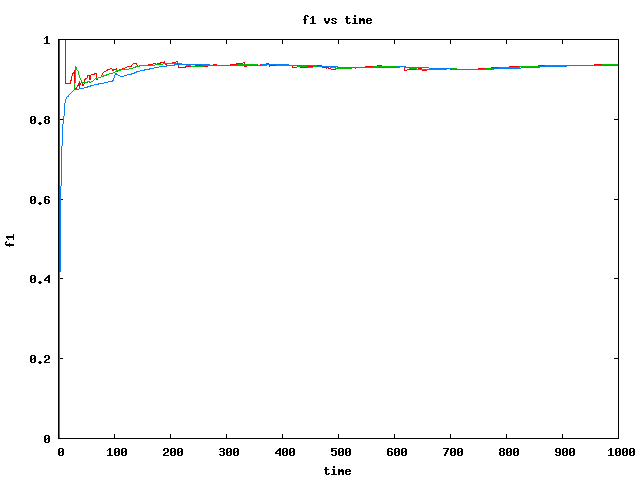
\includegraphics[width=200px]{plots/f1_vs_time.png}
\end{center}

The key takeaway is that our customers are receiving uninterupted, high quality service, and are completely unaware that throughout the experiment our classifier has too little data to generalize well by itself.

The second thing to verify is that we are training a good classifier over time. We held out a dev set of 300 sentences from
the CoNLL NER data that we didn't test on (ie in addition to the 1000 sentences we ran the system on). Every time we retrained
our classifier, we ran it on the this held out dev set, and plot F1. This is to demonstrate that, as expected, we can see
significant improvements in the classifier performance as soon as 1000 sentences in.

\begin{center}
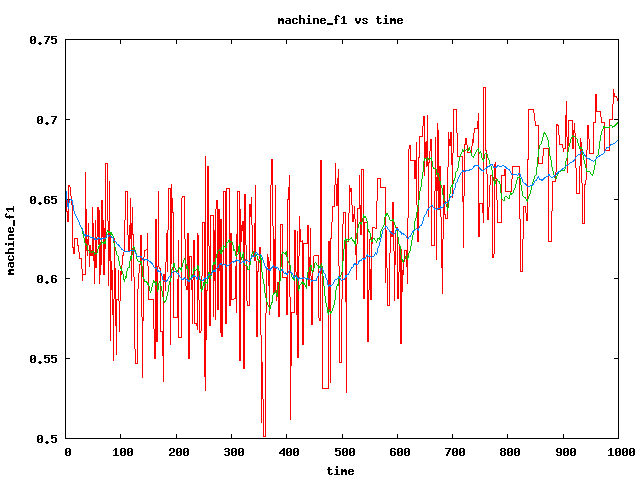
\includegraphics[width=200px]{plots/machine_f1_vs_time.png}
\end{center}

Here the key takeaway is that even though the data we're training this classifier on introduces some noise (we never see
ground truth, just our guesses based on human observations), we are still making our way from 65 to 70 f1 over the course
of only 1000 examples.

The third thing to verify is that our querying behavior is sound.
We don't want to see uniform querying, because that means the system isn't taking advantage of the information in our learned prior.
We also want to see a slight decrease over time, consistent with maintaining high accuracy rates.
This graph plots our queries per sentence on each iteration, normalized by sentence length.

\begin{center}
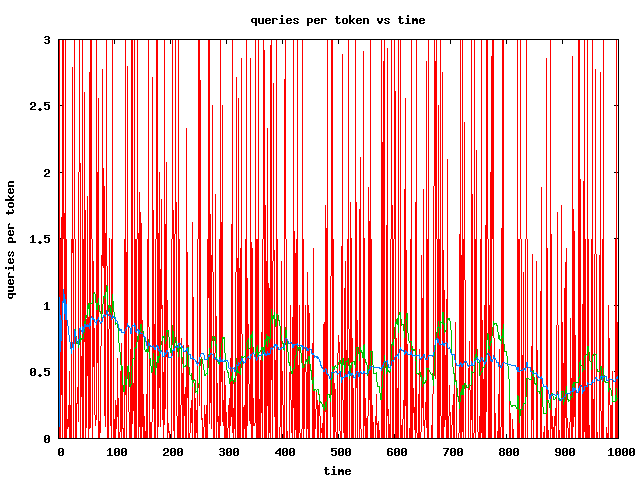
\includegraphics[width=200px]{plots/queries_per_token_vs_time.png}
\end{center}

This plot shows two things. First, there is high variance between sentences on how many queries are needed.
Many sentences come in with such a strong prior that they can be immediately classified, with no need to ask humans.
When querying does take place, it is generally directed towards uncertain tokens.

As a representative example of this querying behavior from the set, take the sentence:

\begin{center}
\textit{``U.S.\ says still committed to Cuba migration pacts.''}
\end{center}

The system, having never seen the token before, starts with a belief that Cuba is 59\% Person, 37\% Location, and 3\% None. The system knows already, from previous learned examples, that ``U.S.'' is a Location with 97\% probability. It immediately fires off two queries about ``Cuba,'' and waits 4 seconds for both responses to return Location. It now believes that ``Cuba'' is a Location with 95\% probability, and decides to turn in its current guess.

\subsection{Movie-review Sentiment Evaluation}

The Stanford Sentiment dataset consists of several thousand highly-polar movie reviews. We select a subset of 1000 of these examples to evaluate our system on.

We start the classifier with 0 examples. We then run the classifier over 1000 examples.

\begin{center}
\begin{tabular}{ | l | r | r | r | r | r | }
    \hline
    \textbf{System} & \textbf{Time/token} & \textbf{Requests/token} & \textbf{Accuracy} \\ \hline
    Human 1-query baseline & TODO & TODO & TODO \\ \hline
    Human 3-query baseline & TODO & TODO & TODO \\ \hline
    Offline baseline & n/a & n/a & 70.03 \\ \hline
    Threshold baseline & TODO & TODO & TODO \\ \hline
    \textbf{Time insensitive MCTS} & TODO & TODO & TODO\\ \hline
\end{tabular}
\end{center}

\subsection{Facial Identification Evaluation}

The Facial Identification dataset is a constructed subset of \todo{Princeton something-or-other}.

\begin{center}
\begin{tabular}{ | l | r | r | r | r | r | }
    \hline
    \textbf{System} & \textbf{Time/token} & \textbf{Requests/token} & \textbf{Accuracy} \\ \hline
    Human 1-query baseline & TODO & TODO & TODO \\ \hline
    Human 3-query baseline & TODO & TODO & TODO \\ \hline
    Offline baseline & n/a & n/a & 70.03 \\ \hline
    Threshold baseline & TODO & TODO & TODO \\ \hline
    \textbf{Time insensitive MCTS} & TODO & TODO & TODO\\ \hline
\end{tabular}
\end{center}

\todo{write}

